%\documentclass[10pt,aspectratio=43,t,l]{beamer}
\documentclass[10pt,aspectratio=169,t,l,fleqn,mathsanserif,sanserif]{beamer}
%\documentclass[10pt]{beamer}

%\setbeamertemplate{footline}[page number]{}

\usepackage{framed}
\usepackage{tcolorbox}
\colorlet{shadecolor}{blue!15}
\usepackage{color,amsmath,xmpmulti,textpos,comment,eurosym,bm,amsthm,tabularx,cancel}
\usepackage{epsfig}
\usepackage{nicefrac}
\usepackage{listings}
%\usepackage{enumitem}
\usepackage{graphicx}    
\usepackage{graphics}
\usepackage{epstopdf}
\usepackage[normalem]{ulem}
\usepackage{float}
%\usepackage[cmbold]{mathtime}
%\usepackage{mt11p}
\usepackage{placeins}
\usepackage{amsmath}
\usepackage{pifont}
\usepackage{color}
\usepackage{amssymb}
\usepackage{mathtools}
\usepackage{subfigure}
\usepackage{multirow}
\usepackage{epsfig}
\usepackage{listings}
%\usepackage{enumitem}
\usepackage{rotating,tabularx}
%\usepackage[graphicx]{realboxes}
\usepackage{graphicx}
\usepackage{graphics}
\usepackage{epstopdf}
\usepackage{longtable}
%\usepackage[pdftex]{hyperref}
\usepackage{breakurl}
\usepackage{epigraph}
\usepackage{xspace}
\usepackage{amsfonts}
\usepackage{eurosym}
\usepackage{ulem}
\usepackage{footmisc}
\usepackage{comment}
\usepackage{setspace}
\usepackage{geometry}
\usepackage{caption}
\usepackage{pdflscape}
\usepackage{array}
\usepackage[round]{natbib}
\usepackage{booktabs}
\usepackage{dcolumn}
\usepackage{mathrsfs}
\usepackage{tikz}
\usetikzlibrary{decorations.pathreplacing}
\usepackage{sansmathaccent}
\pdfmapfile{+sansmathaccent.map}
\usetikzlibrary{shapes.geometric, arrows,chains}
\tikzset{
  startstop/.style={
    rectangle, 
    rounded corners,
    minimum width=3cm, 
    minimum height=1cm,
    align=center, 
    draw=black, 
    fill=red!30
    },
  startsleft/.style={
    rectangle, 
    rounded corners,
    minimum width=3cm, 
    minimum height=1cm,
    align=left, 
    draw=black, 
    fill=red!30
    },
  startsright/.style={
    rectangle, 
    rounded corners,
    minimum width=3cm, 
    minimum height=1cm,
    align=right, 
    draw=black, 
    fill=red!30
    },
  process/.style={
    rectangle, 
    minimum width=3cm, 
    minimum height=1cm, 
    align=center, 
    draw=black, 
    fill=blue!30
    },
  decision/.style={
    rectangle, 
    minimum width=3cm, 
    minimum height=1cm, align=center, 
    draw=black, 
    fill=green!30
    },
  arrow/.style={thick,->,>=stealth},
  dec/.style={
    ellipse, 
    align=center, 
    draw=black, 
    fill=green!30
    },
  font={\fontsize{9pt}{12}\selectfont}
}
%\renewcommand{\labelitemi}{$\blacktriangleright$}

\epstopdfsetup{outdir=./}

\newcolumntype{Y}{>{\centering\arraybackslash}X}
\def\Put(#1,#2)#3{\leavevmode\makebox(0,0){\put(#1,#2){#3}}}

\newcommand{\subhead}[1]{\mbox{}\newline\textbf{#1}\newline}
\newcommand{\ave}[1]{\left\langle #1 \right \rangle}
\newcommand{\eg}{{\it e.g.}}
\newcommand{\ie}{{\it i.e.}}
\newcommand{\cf}{{\it c.f.}}
\newcommand{\etc}{{\it etc.}}
\newcommand{\etal}{{\it et al.}}
%\newcommand{\btVFill}{\vskip0pt plus 1filll}

\newcommand{\del}{D}
\newcommand{\hor}{H}


\newcommand{\Ito}{It\^{o}}
\newcommand{\SP}{S{\&}P500}
\newcommand{\lopt}{\ell_{\text{opt}}}
\newcommand{\gest}{g_{\text{N,T}}}
\newcommand{\elabel}[1]{\label{eq:#1}}
\newcommand{\eref}[1]{Eq.~(\ref{eq:#1})}
\newcommand{\Eref}[1]{Equation~(\ref{eq:#1})}

\newcommand{\flabel}[1]{\label{fig:#1}}
\newcommand{\fref}[1]{Fig.~\ref{fig:#1}}
\newcommand{\Fref}[1]{Figure~\ref{fig:#1}}
\newcommand{\person}[1]{{#1}}
\newcommand{\ra}[1]{\renewcommand{\arraystretch}{#1}}
\newcommand{\vs}[1]{\vspace{.#1cm}}
\newcommand{\vf}{\vspace{.25cm}}
\newcommand{\vff}{\vspace{.6cm}}
\newcommand{\np}{\\ \vf}
\newcommand{\npp}{\\ \vff}
\newcommand{\be}{\begin{equation*}}
\newcommand{\ee}{\end{equation*}}
\newcommand{\bea}{\begin{eqnarray*}}
\newcommand{\eea}{\end{eqnarray*}}
\newcommand{\bc}{\begin{center}}
\newcommand{\ec}{\end{center}}
\newcommand{\bie}{\begin{enumerate}}
\newcommand{\eie}{\end{enumerate}}
\newcommand{\bi}{\begin{itemize}}
\newcommand{\ei}{\end{itemize}}
\newcommand{\toinf}{\rightarrow\infty}
\newcommand{\D}{{\Delta}}
\newcommand{\Dx}{{\Delta x}}
\newcommand{\Dy}{{\Delta y}}
\newcommand{\Du}{{\Delta u}}
\newcommand{\DW}{{\Delta W}}
\newcommand{\DU}{{\Delta U}}
\newcommand{\du}{{\delta u}}
\newcommand{\Dv}{{\Delta v}}
\newcommand{\dt}{{\delta t}}
\newcommand{\gens}{g_{\ave{\,}}}
\newcommand{\ft}[1]{\frametitle{#1}}
\newcommand{\bq}{\begin{quote}}
\newcommand{\eq}{\end{quote}}
\newcommand{\ww}[1]{\bq{\small\rm#1\\}\eq}
\newcommand{\E}{\mathrm{E}}
\newcommand{\Var}{\mathrm{Var}}
\newcommand{\Cov}{\mathrm{Cov}}
\newcommand{\sgn}{\mathrm{sgn}}
\newcommand{\prob}[1]{\mathcal{P}\left(#1\right)}
\newcommand{\lra}{\longrightarrow}
\newcommand{\eps}{\varepsilon}
\newcommand{\ga}{g_\text{ave}}
\newcommand{\gt}{g_\text{typ}}
\newcommand{\gbar}{\bar{g}}
\newcommand{\mbar}{\bar{m}}
\newcommand{\red}[1]{\textcolor{red}{#1}}
\newcommand{\xf}{{x_F}}
\newcommand{\xb}{{x_B}}
\newcommand{\muf}{{\mu_F}}
\newcommand{\mub}{{\mu_B}}
\newcommand{\sigf}{{\sigma_F}}
\newcommand{\sigb}{{\sigma_B}}
\newcommand{\gf}{{\gbar_F}}
\newcommand{\gb}{{\gbar_B}}
\newcommand{\pa}{\textit{pa}}
\newcommand{\taus}{{\tau_\text{s}}}
\newcommand{\Dt}{\Delta t}
\newcommand{\etau}{\tau^\text{eqm}}
\newcommand{\taue}{\tau^\text{EGBM}}
\newcommand{\wtau}{\widetilde{\tau}}
\newcommand{\xN}{\ave{x}_N}
\newcommand{\Sdata}{S^{\text{data}}}
\newcommand{\Smodel}{S^{\text{model}}}
\beamertemplatenavigationsymbolsempty

\newcommand{\tlabel}[1]{\label{tab:#1}}
\newcommand{\tref}[1]{Tab.~\ref{tab:#1}}
\newcommand{\Tref}[1]{Table~\ref{tab:#1}}

\newenvironment{myindentpar}[1]%
{\begin{list}{}%
    {\setlength{\leftmargin}{#1}}%
  \item[]%
}
{\end{list}}

%\usetheme[width=1.8cm,hideothersubsections]{Frankfurt}
\usetheme{Frankfurt}

\newcommand\BackgroundPicture[1]{
\setbeamertemplate{background}{
\parbox[c][\paperheight]{\paperwidth}{
\vfill \hfill
\includegraphics[width=1\paperwidth,height=1\paperheight]{#1}
\hfill \vfill
}}}


\definecolor{lmlblue}{RGB}{0,77,123}
\definecolor{deepblue}{RGB}{35,33,169}
\definecolor{lmllb}{RGB}{237,244,255}
\definecolor{lmlred}{RGB}{155,29,29}
\definecolor{lmlgrey}{RGB}{142,142,142}
\definecolor{lmlgrey2}{RGB}{82,82,82}
\definecolor{grey}{RGB}{210,210,210}
\xdefinecolor{lightblue}{rgb}{0,200,255}
\setbeamercolor{important}{bg=lightblue,fg=red}
\AtBeginEnvironment{definition}{%
  \setbeamercolor{block body}{fg=black,bg=white}
  \setbeamercolor{block title}{bg=lmllb,fg=black}
}

\AtBeginEnvironment{theorem}{%
  \setbeamercolor{block body}{fg=black,bg=white}
  \setbeamercolor{block title}{bg=lmllb,fg=black}
}

%\newcommand{\propnumber}{} % initialize
%\newtheorem*{prop}{Proposition \propnumber}
%\newenvironment{propc}[1]
%  {\renewcommand{\propnumber}{#1}%
%   \begin{shaded}\begin{prop}}
%  {\end{prop}\end{shaded}}
%\AtBeginEnvironment{propc}{%
%  \setbeamercolor{block body}{fg=black,bg=white}
%  \setbeamercolor{block title}{bg=lmllb,fg=black}
%}

\setbeamercolor{fine separation line}{fg=lmllb}

\setbeamercolor{item projected}{fg=white, bg=black}

\setbeamercolor{frametitle}{bg=lmllb, fg=black}
\setbeamertemplate{frametitle}[default][left,colsep=-4bp,rounded=false,shadow=false]

\setbeamercolor{structure}{bg=white, fg=black}
%structure changes color of title in sidebar.

%\setbeamertemplate{frametitle}[default][colsep=-4bp,rounded=false,shadow=false]
\setbeamercolor{section in head/foot}{fg=lmlgrey2, bg=lmllb}
\setbeamercolor{normal text}{fg=black}
\setbeamercolor{title}{bg=white,fg=deepblue}

\hypersetup{colorlinks,linkcolor=,urlcolor=deepblue}

\setbeamerfont{title in sidebar}{size=\fontsize{9}{9}\selectfont}
\setbeamerfont{section in sidebar}{size=\fontsize{7}{7}\selectfont}

% add frame numbers to navigation bar
% (for RSS 2015 conference)
\addtobeamertemplate{navigation symbols}{}{
    \usebeamerfont{footline}
    \usebeamercolor[fg]{footline}
    \hspace{1em}
    \scriptsize
%    \insertframenumber/\inserttotalframenumber
}
\setbeamertemplate{navigation symbols}{} %gets rid of navigation symbols
\setbeamercovered{transparent=20}
%\setbeamertemplate{footline}[frame number] % to show overlay page numbers type: page number
%\setbeamersize{text margin left=0.65cm, text margin right=0.65cm}
%\setbeamercolor{item}{fg=black!70!black} % red bullets
%\setbeamertemplate{itemize subitem}[triangle] % triangle sub-bullets
%\setbeamerfont{itemize/enumerate subbody}{size=\normalsize}


\title[\begin{flushleft} \color{white} {\tiny ???} \end{flushleft}]{\bf {Industrial Organization, Week 1 \\ 
Market power and Efficiency}}
\author[shortname]{ Dio Mavroyiannis \inst{\dag}}
\institute[\begin{flushleft} \color{white} {\large ???} \end{flushleft}]{Milestone Institute}
%\institute[shortinst]{\inst{*} London Mathematical Laboratory \and \inst{\dag} Universit\'{e} Paris-Dauphine \and \inst{\ddag} London Mathematical Laboratory and Santa Fe Institute}
\date{03 February 2021}

\AtBeginSection[]{
\frame{
\ft{Agenda}
\tableofcontents[currentsection,hideallsubsections]
}
}

\makeatletter
\setbeamertemplate{headline}{%
  \pgfuseshading{beamer@barshade}%
  \ifbeamer@sb@subsection%
    \vskip-9.75ex%
  \else%
    \vskip-7ex%
  \fi%
    \begin{beamercolorbox}[ht=3.5ex,dp=2.125ex]{section in head/foot}
     \insertsectionnavigationhorizontal{\textwidth}{}{}%
  \end{beamercolorbox}%
  \ifbeamer@sb@subsection%
    \begin{beamercolorbox}[ignorebg,ht=2.125ex,dp=1.125ex,%
      leftskip=.3cm,rightskip=.3cm plus1fil]{subsection in head/foot}
      \usebeamerfont{subsection in head/foot}\insertsubsectionhead
    \end{beamercolorbox}%
  \fi%
}%

\makeatother

\setbeamertemplate{mini frames}{}
\setbeamertemplate{itemize items}[triangle]

\begin{document}

\frame{\titlepage\insertlogo}

%%%%%%%%%%%%%%%%%%%%%%%%%%%%%%%%%%%%%%%%%%%%%



\section{Power}

\frame{\ft{Nuts and bolts: Market power and formal market power}

\setbeamertemplate{itemize items}[triangle]
\bi
\item \textbf{Power}: The ability to acquire goods below their market price
\item \textbf{Market power}: Market power is the ability to set prices above cost.
\item Memo on cost: Costs subjective, depends on the uneasiness of the process of creation(think actors/writers)
\item \textbf{Formal Market power}: r = (R-C)/C or if costs proportional to output then: $r = (P-UC)/UC$
\item \textbf{Effects for firms}: More profits
\item \textbf{Effects for consumers}: Value transfer from consumer to firm
\ei

}


\frame{\ft{Nuts and Bolts 2: Static/Dynamic and Sources of market power}

\setbeamertemplate{itemize items}[triangle]
\bi
\item \textbf{Static effects:} Effects that happen outside of time(axiomatic)
\item Example: \{What is the equilibrium? How is the equilibrium affected by X \}
\item \textbf{Dynamic:} Effects that happen over time(empirical)
\item Example: \{How do we get to equilibrium? How do profits change over time?, \}
\item \textbf{Intellectual property:} Gives a legal monopoly over 20 years
\item Gives market power in the short run, but good in the long run(investment)
\item \textbf{Regulation:} Limiting prices or quantities or product variety
\item Limits investments and allocations
\item \textit{Both of these are special cases of barriers to exit and entry}
\ei

}


\section{Efficiencies}

%%%%%%%%%%%%%%%%%%%%%%%%%%%%%%%%%%%%%%%%%%%%%

\frame{\ft{Types of efficiencies}

\setbeamertemplate{itemize items}[triangle]
\bi
\item \textbf{Allocational efficiency}: The highest valuation person gets the item
\item \textbf{Investment efficiency}: Bringing goods into existence/market
\item \textbf{Production efficiency}: Lower costs
\item \textbf{Rent-seeking efficiency}: Unproductive use of resources(think bureaucracy)
\ei


}


\section{Examples}

%%%%%%%%%%%%%%%%%%%%%%%%%%%%%%%%%%%%%%%%%%%%%


\frame{\ft{Occupational Licensing}


\begin{picture}(80,80)(0,0) %syntax: \begin{picture}(width,height)(x-offset,y-offset)
\put(140,-60){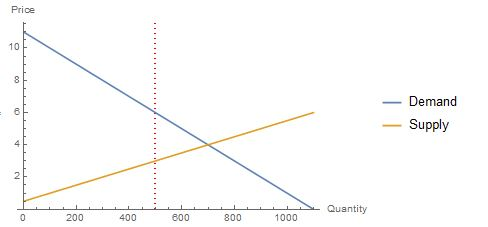
\includegraphics[width=10.5cm]{./IO_Week1_SD_occ.jpg}}
\end{picture}

\setbeamertemplate{itemize items}[triangle]
\bi
\item - Allocational efficiency
\item $\downarrow$  Investment
\item $\downarrow$  Production
\ei

}



\frame{\ft{Price control(min)}


\begin{picture}(80,80)(0,0) %syntax: \begin{picture}(width,height)(x-offset,y-offset)
\put(120,-60){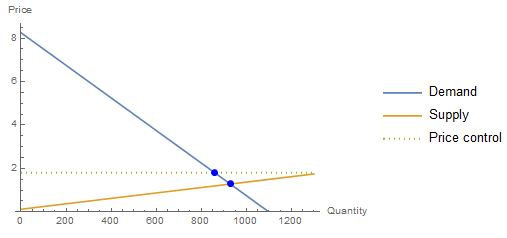
\includegraphics[width=10.5cm]{./IO_Week1_SD_pcmin.jpg}}
\end{picture}

\setbeamertemplate{itemize items}[triangle]
\bi
\item - allocational
\item $\downarrow$ investment
\ei

}

\frame{\ft{Price control(max)}


\begin{picture}(80,80)(0,0) %syntax: \begin{picture}(width,height)(x-offset,y-offset)
\put(120,-60){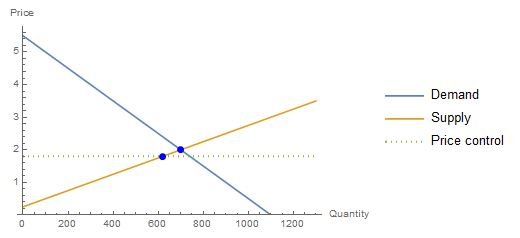
\includegraphics[width=10.5cm]{./IO_Week1_SD_pcmax.jpg}}
\end{picture}

\setbeamertemplate{itemize items}[triangle]
\bi
\item $\downarrow$ allocational
\item $\downarrow$ investment
\ei

}

\frame{\ft{Monopsony}


\begin{picture}(80,80)(0,0) %syntax: \begin{picture}(width,height)(x-offset,y-offset)
\put(120,-60){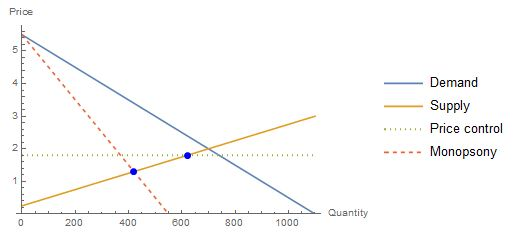
\includegraphics[width=10.5cm]{./IO_Week1_SD_monopsony.jpg}}
\end{picture}

\setbeamertemplate{itemize items}[triangle]
\bi
\item - allocational
\item $\uparrow$ investment
\ei

}

% It is worth emphasizing that all costs are generated through a subjective process. Whether the cost to consume something is 1 dollar or 10 dollars depends on whether the process to create or extract that good is something people want to do or not. This explains why actors/writers often get paid less, their work is more enjoyable.
\frame{\ft{How do we do industrial organization? }


\setbeamertemplate{itemize items}[triangle]
\bi
\item Describe a market structure: Who are the buyers and sellers, what are the characteristics of the good and how does that affect their interaction. What are the strategies of the buyers and sellers? 
\item Does the environment cause the strategy of vice versa? 
\item How much can we explain with positing a market structure? 
\item \textbf{Economics is more about what we cannot say}: 
\item Supply and Demand: We cannot reason from a price change
\item Bertrand Paradox: We cannot measure competition from the number of players 
\ei

}



\frame{\ft{Some notes on homework}


\setbeamertemplate{itemize items}[triangle]
\bi
\item Step 1: Equalize quantity demanded with quantity supplied
\item Step 2: Solve for price
\item Step 3: Plug the price into the equations to get the quantity
\item Step 4: Draw a graph
\item Step 5: If there is a tax, compute the amount collected(tax*quantity)
\item Step 6: Compute the area of the upper triangle(consumer surplus)
\item Step 7: Compute the area of the lower triangle(producer surplus)
\item Step 8: Add 5, 6, 7 for total surplus
\item Step 9: Deadweight loss: is the surplus difference with and without taxation
\ei

}


\end{document}